\documentclass[output=paper]{langsci/langscibook}
\ChapterDOI{10.5281/zenodo.3972848}

\author{Norma Schifano\affiliation{University of Birmingham}\lastand Federica Cognola\affiliation{La Sapienza University, Rome}}

\title{From macro to nano: A parametric hierarchy approach to the diatopic and
diachronic variation of Italian \textit{ben}}

% \chapterDOI{} %will be filled in at production

\abstract{In this squib we discuss the morpho-syntactic requirements affecting
    the distribution of the \ili{Italian} discourse particle \emph{ben} (lit.\
    ‘well’) as employed in a selection of regional varieties of the language.
    We present a preliminary comparison with its attestations in earlier stages
    of the language and we show how the attested diatopic and diachronic
    variation may be modelled in terms of a parameter hierarchy of the type
    developed by the \emph{ReCoS} team.}

\maketitle

\begin{document}\glsresetall

\rohead{\thechapter\hspace{0.5em}From macro to nano}

\section{Introduction}

The aims of the following squib are: (i) introducing the morpho-syntactic
requirements affecting the distribution of a poorly studied discourse particle,
namely \ili{Italian} \emph{ben} (lit.\ ‘well’), as employed in a selection of
regional varieties of the language, building on the work in
\textcite{CognSchi2015,CognSchi2018b,CognSchi2018} (\Cref{sec:23-diatopic}),
(ii)~presenting a preliminary comparison with its attestations in earlier
stages of the language (\Cref{sec:23-diachronic}), and (iii) showing how the
attested diatopic and diachronic variation are particularly relevant for our
understanding of comparative syntax in that, far from being random, they fit
the predictions of the parametric hierarchy approach, as developed by the
\emph{ReCoS} team
(\citealt{Roberts2012,BibRob2012,BibRob2015,BibRob2016,BibHolRobShee2014,BibRobShee2014},
a.o.; \Cref{sec:23-hierarchy}).

The challenge raised by the behaviour of this element is twofold. On the one
hand, particles represent a \enquote{poorly understood group of elements}
\parencite[387]{BibShee2011} which raise a number of both empirical and
theoretical questions, including i.a.\ a proper understanding and adequate
description of their individual syntactic functions, of their (lack of)
ordering restrictions, as well as defectivity, optionality, degree and path of
grammaticalization and pragmaticalization, semantic contribution, etc.
\parencite{BibShee2011,BibHaevanKem2014}. On the other hand, the sub-category
of \emph{discourse} particles introduces a number of even more complex
issues.\footnote{A wider related issue concerns the notion of \enquote{discourse}
    itself, which is too vast for us to be able to discuss it here.  The reader
    is referred to \citet{BayHinTro2015} for an updated overview of some of the
most prominent proposals about its codification and relationship with syntax.}
According to \citegen[2012]{Zimmermann2011} semantic criterion, discourse
particles can be defined as \enquote{expressions [which] contribute only to the
expressive content of an utterance, and not to its core propositional content}
(cf.\ also \citealt[450]{BayObe2011}, a.o.). This means that any formalization
of discourse particles must be able to capture not only their syntactic
behaviour and structural status (as, for example, (deficient) \isi{adverbs},
\citealt{Cardinaletti2011,Cardinaletti2015,Manzini2015}; TP pro-forms,
\citealt{HaeWei2015}; speech act functional heads\is{functional items},
\citealt{Haegeman2014,Hill2014}; propositional anaphors, \citealt{HinMun2015}), but also
their discourse properties, which involve highly heterogeneous non-syntactic
categories such as speakers’ \enquote{emotional needs} (\citealt{Gabelentz1969}; cf.\
i.a. the expression of commitment, e.g.\ \ili{German} \emph{wohl},
\citealt{Zimmermann2011}; confidence, e.g.\ \emph{ben} in some varieties of
\ili{Italian}, \citealt{Coniglio2008,Cardinaletti2011}; surprise, e.g.\ Cantonese
\emph{me1}, \citealt{Li2006}; surprise-disapproval, e.g.\ \ili{Bangla} \emph{ki},
\citealt{Bayer1996}; concern, e.g.\ \ili{German} \emph{denn}, \citealt{BayObe2011};
impatience, e.g.\ Dolomitic \ili{Ladin} \emph{po}, \citealt[52]{Hack2014}) or context\slash
common ground dependence (cf.\ i.a.\ presupposition, e.g.\ \ili{Italian}
\emph{mica}, \citealt{Cinque1976}, \citealt{Zanuttini1997}; existence of mutual
knowledge, e.g.\ \ili{German} \emph{ja}, \citealt{Zimmermann2011}; evidentiality,
e.g.\ Bellunese \emph{lu}/\emph{ti}/\emph{mo}/\emph{po}, \citealt{HinMun2015}),
just to mention a few.

In what follows, we leave these issues aside, simply assuming that \ili{Italian}
\emph{ben} is a discourse particle located in the IP area (see further
discussion in \citealt{CognSchi2018b,CognSchi2018}).\footnote{As for the
    syntactic status of \emph{ben}, the reader is referred to
    \textcite{CognSchi2015,CognSchi2018b,CognSchi2018}, where \emph{ben} is
    analysed as a weak XP (in the sense of \citealt{CarSta1999}), as it is
    subject to the series of syntactic restrictions affecting weak elements
    (e.g.\ impossibility of fronting, coordination, focusing\is{focus}) which do not
    extend to \emph{ben(e)} when used as a manner adverb. More specifically, we
    assume that when it is used as a discourse particle, \emph{ben} is licensed
    in NegPresuppositionalP by a silent negative operator in ForceP and
    receives its presuppositional character by a Focus in PolarityP (see
    \citealt{Hernanz2010} for the role of PolarityP in the licensing of \ili{Spanish}
    \emph{bien}). Also note that, according to the above definition of
    discourse particles (also called \emph{modal particles} in the literature
    due to their semantics and position in the clause, see
    \citealt{Weydt1969}), these elements have to be kept distinct from
    so-called conversational-management elements, in that the latter have a
    pragmatic function similar to discourse particles, but are typically hosted
    in the CP layer. Interestingly, the \ili{Italian} manner adverb \emph{bene/ben}
    has also developed an usage as a conversational-management element (cf.\
\emph{be’}).} Conversely, we focus our attention on the diatopic
distribution of this element, as this proves to be particularly interesting in
that it is subject to an increasing set of morpho-syntactic restrictions which
reflect the macro > meso > micro > nano typology of parameters of the kind
advocated by the \emph{ReCoS} approach.  Accordingly, we claim that the
fine-grained diatopic variation which affects \ili{Italian} \emph{ben} can be
modelled in terms of a parameter hierarchy,\is{parameter hierarchies} which allows us to gain insights
also into the diachronic development of this element. The case of \ili{Italian}
\emph{ben} thus provides evidence that the adequacy of the parametric hierarchy
approach stretches to (the morpho-syntactic behaviour of) elements at the
syntax-discourse interface.

\section{Italian: Diatopic variation in morpho-syntactic requirements}\label{sec:23-diatopic}

Consistently with the cross-linguistic behaviour of manner \isi{adverbs}, which are
known to have developed  homophonous forms with a discourse value both in
Romance (\citealt{Belletti1990,Belletti1994,Lonzi1991,Cinque1976,Cinque1999,%
Vinet1996,WalDet2007,Coniglio2008,Hernanz2010,Cardinaletti2011,PadPen2014},
a.o.) and Germanic (\citealt{Weydt1969,Baardewyk-Resseguier1991}, a.o.), the
Italian manner adverb \emph{ben(e)} ‘well’ (\ref{ex:schifano:12.1}a,b) co-exists with the
non-adverbial element \emph{ben} (\ref{ex:schifano:12.1}c), which has been traditionally described
as conveying an em\-phat\-ic/as\-sertive meaning, used to
reinforce the assertion (\citealt{Belletti1990,Belletti1994,Lonzi1991}) and
to express speakers’ confidence about the propositional content of their
assertion (\citealt{Coniglio2008}; \citealt{Cardinaletti2011}):\footnote{The
    translation of \emph{ben} in (\ref{ex:schifano:12.1}b) is the one offered in the cited work. On
    the whole, \emph{ben} does not seem to have an immediate corresponding form
    in English, where it could at best be rendered with an emphatic stress on
    the verb or as \emph{indeed}. As such, it will not be translated in the
examples below coming from our corpus of contemporary \ili{Italian}, while it will be
rendered with various periphrases in the early examples, according to the
context.}

\ea\label{ex:schifano:12.1} \ili{Italian} \parencite[171, fn.\ 20]{Cinque1999}
	\ea
		\gll    Carlo disegna \textit{bene}.\\
			    C.  draw.\Prs{}.\Tsg{}  well\\
        \glt    \enquote*{Carlo is good at drawing.}
	\ex
		\gll    Carlo è una persona \textit{ben} educata.\\
			    C.  be.\Prs.\Tsg{} a person well  educated\\
        \glt    \enquote*{Carlo is a well-educated person.}
    \ex
		\gll    Avrai \textit{ben} già cenato.\\
			    have.\Fut{}.\Ssg{} \textsc{ben} already dined\\
        \glt    \enquote*{You will have indeed already eaten.}
	\z
\z

In \textcite{CognSchi2018b,CognSchi2018}, we have argued instead that the core
property of \ili{Italian} \emph{ben} is that of denying the interlocutor’s negative
presupposition (cf.\ also \citealt{WalDet2007} on French and
\citealt{Hernanz2010} on \ili{Spanish}), i.e.\ \emph{ben} can only occur in
(syntactically positive) contexts in which the negative counterpart of the
proposition expressed by the sentence is part of the common ground (cf.\
\citealt{Cinque1976} on \emph{mica}):

\ea \ili{Italian}
	\ea Speaker A: (negative presupposition)\\
		\gll    Nicola non l’avrebbe neanche toccata quella roba.\\
			    N. not it=have.\Cond{}.\Tsg{} even touched that stuff\\
        \glt    \enquote*{Nicola wouldn’t even have touched that stuff.}
	\ex Speaker B: (negative presupposition denied)\\
		\gll    Nicola l’avrebbe \textit{ben} mangiata la carne.\\
			    N. it=have.\Cond{}.\Tsg{} \textsc{ben} eaten the meat\\
        \glt    \enquote*{Nicola would have eaten the meat.}
	\z
\z

In order to shed further light on the behaviour of this element, we collected
data with native speakers and we found that regional varieties of \ili{Italian} can
be classified into three main groups, in accordance with the morpho-syntactic
requirements exhibited by \emph{ben}, i.e.\ Group 1 (Trentino), Group 2 (mainly
Venetan varieties) and Group 3 (Rovigo, plus localities in Friuli Venezia
Giulia, Lombardy, Piedmont, Emilia Romagna, Lazio, Marche and Puglia).

Looking at the morpho-syntactic requirements in more detail, the following
restrictions can be identified:\footnote{The following morpho-syntactic
    restrictions were identified through a questionnaire run with 28 speakers
    of mixed age, gender and education from 15 different localities, who were
    asked for grammaticality judgements on a 1--5 scale on 67 sentences
    testing the occurrence of \emph{ben} across a variety of verb forms and
    \gls{TAM} contexts (see \citealt{CognSchi2018b,CognSchi2018} for details).
    The reader is referred to the aforementioned works for a discussion of one
    additional morpho-syntactic restriction which was identified for Group 3
    (cf.\ a preference for transitive over unaccusative verbs) and a difference
    in the interpretative requirements of \emph{ben} between Group 1 and 3
    (cf.\ negation of implicit vs explicit negative presupposition).}

\newpage

\ea\label{ex:schifano:12.3} Morpho-syntactic requirements on the distribution of
        \emph{ben}
	\ea embedded non-root contexts are ruled out (Restriction 1);
    \ex \gls{TAM} combinations not involving a non-finite form are ruled out
        (Restriction 2);
    \ex among restructuring verbs, \emph{potere} ‘can’ is widely accepted,
        \emph{volere} ‘want’ is more restricted and
        \emph{smettere} ‘stop’ is largely ruled out (Restriction 3);
	\z
\z

While all the three restrictions apply to Group 3, Group 1 is only subject to
Restriction 1.\footnote{Note however that, for all speakers, \emph{ben} can be
used in root-like embedded clauses, like in embedded clauses introduced by a
verbum dicendi.}  By way of illustration, consider the examples below,
showing that embedded non-root contexts like the ones selected by a matrix
volitional verb are ruled out in both groups (\ref{ex:schifano:12.4}); while both simple and
compound tenses are admitted by Trentino speakers, only the latter combination
is admitted by speakers of Group 3 (\ref{ex:schifano:12.5}); while Trentino allows \emph{ben} to
occur with \emph{potere}\slash\emph{volere}\slash\emph{smettere}, only the former is
completely grammatical in all the tested contexts in Group 3 (\ref{ex:schifano:12.6}):\footnote{See
further examples in \textcite{CognSchi2018b,CognSchi2018}.}

\ea\label{ex:schifano:12.4} Group 1\slash3 (Italian)\\
	\ea[*]{
        \gll   Gianni vuole che Marco compri \textit{ben} qualcosa per cena.\\
			    G. want.\Prs.\Tsg{} that M. buy.\Sbjv{}.\Tsg{} \textsc{ben} something for dinner\\
        \glt    \enquote*{Gianni wants Marco to buy something for dinner.}}\label{ex:schifano:12.4a}
	\ex[*]{
        \gll    Gianni avrebbe voluto che Marco avesse \textit{ben} comprato
        qualcosa per cena.\\
			    G. have.\Cond{}.\Tsg{} wanted that M. have.\Sbjv.\Ipfv.\Tsg{} \textsc{ben} bought something for dinner\\
		\glt    \enquote*{Gianni would have wanted Marco to buy something for
                dinner.}}\label{ex:schifano:12.4b}
	\z
\ex \label{ex:schifano:12.5} \ili{Italian}
	\ea\label{ex:schifano:12.5a} Group 1\slash *3\\
		\gll    Gianni compra \textit{ben} qualcosa per cena quando può.\\
			    G. buy.\Prs.\Tsg{} \textsc{ben} something for dinner when can.\Prs.\Tsg{}\\
		\glt    \enquote*{Gianni buys something for dinner when he
        can.}\newpage
	\ex\label{ex:schifano:12.5b} Group 1\slash3\\
		\gll    Gianni avrebbe \textit{ben} comprato qualcosa per cena, se
        avesse potuto.\\
			    G. have.\Cond{}.\Tsg{} \textsc{ben} bought something for dinner if have.\Sbjv.\Ipfv.\Tsg{} been.able\\
		\glt    \enquote*{Gianni would have bought something for dinner if he had been able to.}
	\z
\ex \label{ex:schifano:12.6} Group 3 (Italian)\\
	\ea[]{
        \gll    Gianni può \textit{ben} parlare con la povera Maria.\\
			    G. can.\Prs.\Tsg{} \textsc{ben} speak.\Inf{} with the poor M.\\
        \glt    \enquote*{Gianni should speak with Mary, poor thing.}}
	\ex[]{
        \gll    Gianni *vuole / vorrà \textit{ben} incontrare Rihanna.\\
                G. \hphantom{*}want.\Prs.\Tsg{} {} want.\Fut.\Tsg{} \textsc{ben}  meet.\Inf{} R.\\
        \glt    \enquote*{Gianni wants / will want to meet with Rihanna.}}
	\ex[*]{
        \gll    Gianni smette \textit{ben} di fumare ogni volta che gli=dicono
        che fa male.\\
			    G. stop.\Prs.\Tsg{} \textsc{ben} of smoke.\Inf{} every time that \Tsg{}.\Dat{}=say.\Prs{}.\Tpl{} that do.\Prs.\Tsg{} harm\\
		\glt    \enquote*{Gianni quits smoking every time they tell him that it
                is harmful.}}
	\z
\z

On the basis of the distributional facts summarised above, we classify Trentino
as the productive isogloss for the use of \emph{ben}. Conversely, Group 3
allows a considerably more restricted usage and Group 2 represents a
transitional area between the two, where the above restrictions do not apply
consistently yet. One of the most striking results of this investigation is
that the localities in Group 3 behaved surprisingly homogeneously, in spite of
their geographical scatteredness, suggesting that once outside the productive
isogloss, any varieties conform to the same behaviour. In what follows, we
shall not attempt at accounting for the above restrictions (see
\citealt{CognSchi2018b,CognSchi2018} for a proposal), but we will instead
consider a representative set of examples regarding the distribution of this
particle in earlier attestations of \ili{Italo-Romance} in order to assess whether
the more liberal pattern of Trentino instantiates an innovative or conservative
stage in the distribution of \emph{ben}.

\section{Italian: Diachronic variation in morpho-syntactic
requirements}\label{sec:23-diachronic}

A preliminary examination of occurrences of \emph{ben} in earlier attestations
of \ili{Italo-Romance} suggests that the extensive use of Trentino reflects a
conservative stage, where \emph{ben} occurred in a wider range of \gls{TAM}
contexts than present-day (standard) \ili{Italian}.\footnote{We take
    \enquote{standard} \ili{Italian} to pattern with Group 3, as shown by the scores
    provided by our central-southern informants, whose judgements refer to
    their competence of the standard language, \emph{ben} being absent both
    from their regional varieties of \ili{Italian} and their local \ili{Romance} dialects.
    The diachronic data reported below are taken from two central-northern
    varieties only, namely Old Tuscan (cf.\ \emph{Novellino}, about end of the
    13th
    century) and Old Venetan (cf.\ \emph{Lio Mazor}, 14th century). We therefore
    do not exclude the possibility that other early varieties of \ili{Italo-Romance}
    behave differently.  The English translation provided for \emph{Novellino}
    have been freely adapted from \citegen{Consoli1997} edition.} More
    specifically, we observe that (i) the particle was already employed to deny
    a negative presupposition, and (ii) although occurrences of \emph{ben} in
    non-root embedded contexts do not seem to be attested (cf.\ Restriction
    1),\footnote{That \emph{ben} should be excluded from non-root embedded
        contexts also in the early varieties under review here is not
        surprising under the analysis proposed in \textcite{CognSchi2018b},
    where \emph{ben} is licensed by a negative operator in ForceP, as argued
elsewhere for other discourse particles (see \citealt{Coniglio2008} and
\citealt{Zimmermann2004,Zimmermann2011}, a.o.).} the particle was not only
allowed with compound tenses, such as the present perfect (\ref{ex:schifano:12.7}a) and pluperfect
indicative (\ref{ex:schifano:12.7}b), as well as with restructuring verbs like \emph{potere} ‘can’
(\ref{ex:schifano:12.7}c), but was also readily admitted with simple tenses, such as the present
indicative (\ref{ex:schifano:12.8}), the imperfect indicative (\ref{ex:schifano:12.9}), the simple past (\ref{ex:schifano:12.10}) and the
simple future (\ref{ex:schifano:12.11}), on a pair with modern-day Trentino and unlike the
contemporary \ili{Italian} varieties of Group 3 (cf.\ Restriction 2):\footnote{We
leave it open to future research to determine whether Restrictions 3 was active
or not in the early varieties under investigation here.}

\ea\label{ex:schifano:12.7}
    \ea (negative presupposition: the knight does not deserve to be treated in
        such an uncivil manner)\\
        \begin{otherlanguage}{italian}
        Così tenendo lor camino, trovaro il re
        Meliadus ch’andava a uno torneamento, altressì a guisa di cavaliere errante
        e sue arme coverte. E’ domandò questi sergenti: “Perché menate voi a ‘mperatore
        questo cavaliere? E chi [è] elli, che cosìe lo disonorate villanamente?” Li
        sergenti rispuosero: “Elli hae \textit{bene} morte servita; e se voi il sapeste
        come [noi], voi il menareste assai più tosto di noi. Adomandatelo di suo
        misfatto!”
        \end{otherlanguage}\hfill(\emph{Novellino}, LXIII, p.267, l.20--28)\\
        \enquote*{Along the road they met King Meliadus, on his way to a tournament,
        also dressed as a knight errant and hiding his weapons. He asked the
        vassals: ``Why are you carrying this knight to the emperor? And who is
        he, that you are dishonouring him in such an uncivil manner?'' The
        vassals replied: ``He well deserves to die; and if you knew why, you
        would be carrying him faster than us. Ask him yourself about his
        crime!''}
    \ex (context: there is a quarrel involving Lena’s son and Pero Stomarin.
        Lena’s son was supposed to give Pero Stomarin money for the fish, but
        according to Çanun he has kept it for himself. Negative presupposition:
        Lena’s son has not given the money to Pero Stomarin)\\
        \begin{otherlanguage}{italian}
        \relax[\dots] la quala dis che Çanun diseua che lo fio de Lena aueua
        toleto li deneri del pes da Siluester Uener et lo fio dis ch’el li
        aueua \textit{ben} dati a Pero Stomarin.
        \end{otherlanguage}\hfill
        (\emph{Lio Mazor}, p.48, l.160--163)\\
        \enquote*{[\dots] she said that Çanun said that Lena’s son had taken
        the money for the fish from Siluester Uener and the son said that
        he had indeed given it to Pero Stomarin.}
    \ex (negative presupposition: the infant girl cannot be the doctor’s
        daughter)\\
        \begin{otherlanguage}{italian}
        Uno medico di Tolosa tolse per mogliera una gentile donna di
        Tolosa, nepote dell’arcivescovo. Menolla. In due mesi fece una
        fanciulla. Il medico non ne mostrò nullo cruccio, anzi consolava la
        donna e mostravale ragioni secondo fisica, che \textit{ben} poteva
        esser sua di ragione [\dots{}].
        \end{otherlanguage}\hfill
        (\emph{Novellino}, XLIX, p.234, l.3--7)\\
        \enquote*{A doctor from Toulouse took for his wife a gentle woman of Toulouse,
        the niece of the Archbishop. He brought her home. Two months later she
        gave birth to an infant girl. The doctor showed no signs of anger,
        instead he consoled his lady and presented many reasons, according to
    the law of physics, which logically proved the child could be his.}
	\z
\ex \label{ex:schifano:12.8}(negative presupposition: your god is not better)\\
    \begin{otherlanguage}{italian}
            E tornando al signore per iscommiatarsi da lui, il
            signore disse: – Or sei tu ancor qui? Non avestu la torta? – Messer
            sì, ebbi. – Or che ne facesti? – Messere, io avea allora mangiato:
            diedila a un povero giullare che mi diceva male perch’io vi
            chiamava mio Iddio. – Allora disse il signore: – Va’ con la mala
    ventura: ché \textit{bene} è miglior il suo Iddio che ‘l tuo! – E disseli
    il fatto della torta.
    \end{otherlanguage}\hfill
    (\emph{Novellino}, LXXIX, p.309, l.30--39)\\
    \enquote*{[the minstrel] returned to his lord to formally take his leave,
    and his lord said: -- You’re still here? Didn’t you receive a tart?
    -- Sire, I had it -- What did you do with it? -- Sire, I had already
    eaten: I gave it to that poor minstrel who chided me for calling you my
    god. -- Then the lord said: May misfortune follow you, for it is true that
    his god is better than yours! -- And then he told him all about the tart.}
\ex \label{ex:schifano:12.9}
    (context: a watchman sees a boat in the sea which looks like Nasel’s one.
    The watchman orders the man on the boat to dock, but the person refuses and
    gets a fine. The judge asks the watchman whether he knows the man on the
    boat and the watchman replies no. Negative presupposition: the boat was not
    Nasel’s)\\
    \begin{otherlanguage}{italian}
    Domandà s’el lo cogno[se]se, li dis, no; mo lo burclo
    era \textit{ben} del Nasel.\end{otherlanguage}\\
	(\emph{Lio Mazor}, p.43, l.11)\\
    \enquote*{[the judge] asks whether he knows [the man on the boat], he says
    ``no''; but the boat was indeed Nasel’s.}
\ex \label{ex:schifano:12.10}
	(negative presupposition: you didn’t see them passing)\\
    \begin{otherlanguage}{italian}
    Quell’altro cavalcò poi più volte, tanto che udì il
    padre e la madre fare romore nell’agio, e intese dalla fante com'ella
    n’era andata in cotal modo. Questi sbigottì: tornò a’ compagni e disselo
    loro. E que’ rispuosero: – \textit{Ben} lo vedemmo passar con llei, ma nol
    conoscemmo: et è tanto, che puote bene essere allungato; et andarne per cotale
    strada.
    \end{otherlanguage}\\
	(\emph{Novellino}, XCIX, p.350, l.47--53)\\
    \enquote*{The other man rode past her house many times, until he heard her
    mother and father making a ruckus inside, and he learned from the
    maidservant what had taken place. He was mortified: he returned to his
    companions and told them all \emph{[i.e.\ that the lady had left with
    another man, without being seen]}. They replied: -- We did see him pass
    with her, but we didn’t recognise him: and it was so long ago, they
    must be far away by now; this is the road they took.}
\ex \label{ex:schifano:12.11}
    (context: there is a quarrel involving Maria, Magdalena and Francesca.
    Maria wants to buy some bread from Magdalena. She takes a piece of bread,
    but another woman, Francesca, grabs it from her hands. There is a fight
    between the two women. Magdalena understands that Maria wants to steal the
    bread and Maria answers as below. Negative presupposition: you will not pay
    for the bread)\\
    \begin{otherlanguage}{italian}
    \relax[\dots] no me-lo tor, ch’e’ tel pagarò
    \textit{ben}.
    \end{otherlanguage}\hfill
	(\emph{Lio Mazor}, p.27, l.12)\\
    \enquote*{don’t take it away from me, that I will indeed pay you for that}
\z

The availability of \emph{ben} across a wide selection of \gls{TAM} contexts
(vs.\ Restriction 2) exemplified in (\ref{ex:schifano:12.8}--\ref{ex:schifano:12.11}) points to a high degree of
grammaticalization of this particle in earlier stages of \ili{Italo-Romance}, a
situation which today persists in Trentino, i.e.\ the productive isogloss, but
not elsewhere.\footnote{Here we are also glossing over the (apparently)
    distinct placements of \emph{ben} in the examples (\ref{ex:schifano:12.8}--\ref{ex:schifano:12.11}), including its
    preverbal placement (cf.\ \ref{ex:schifano:12.7}c, \ref{ex:schifano:12.8}, \ref{ex:schifano:12.10}, which have to be interpreted in
    the light of the distinct word order restrictions which were active in
    earlier varieties of \ili{Italo-Romance} (see \citealt{Ledgeway2012} for an
    overview and references) and which are not immediately relevant for the
    purposes of the present discussion. We leave it open to further research to
    determine the exact position of \emph{ben} in early \ili{Italo-Romance} varieties
    and to establish whether the analysis offered by
    \textcite{CognSchi2018b,CognSchi2018} can capture this variation. We also
    note, in passim, that the full form \emph{bene} too was allowed in its
    discourse particle meaning (\ref{ex:schifano:12.7}a), (\ref{ex:schifano:12.8}), unlike in present-day regional
Italian.} Accordingly, we suggest that the distribution of \emph{ben} in
Trentino reflects a conservative pattern. The reason why Trentino has preserved
an earlier stage of the language, unlike all the other varieties of the \ili{Italian}
peninsula under investigation here, may be linked to the contact with \ili{German}
(in terms of reinforcement of a shared property, see \citealt{Beninca1994,%
Cordin2011,Cognola2014}), which makes a very productive use of discourse
particles (see \citealt{CognSchi2018} for a parallel between \ili{Italian} \emph{ben}
and \ili{German} \emph{doch} and \citealt{Weydt1969}, among many others, on \ili{German}
discourse particles). As for the other varieties, these show a reduced
distribution of \emph{ben} which, from a diachronic perspective, may be
interpreted as an example of retraction \citep{Norde2011}, i.e.\ it also
reflects the steps of a diachronic process whereby \emph{ben} was originally
allowed in all the contexts admitted in early \ili{Italo-Romance} and still retained
by Trentino. Our fine-grained diatopic investigation has shown that, despite
their geographical scatteredness, all the speakers outside the productive
isogloss are remarkably consistent in their judgements. We take this to
indicate that the retraction of \emph{ben} from early \ili{Italo-Romance} to the
present-day varieties outside the productive isogloss has followed the same
path. This diatopic and diachronic path can be informally represented as in
(\ref{ex:schifano:12.12}):\footnote{Note that the geographical factor is not totally irrelevant
    here, as localities closer located to Trentino (see varieties in the
transitional Group 2 like Cortina D’Ampezzo) allow \emph{ben} in a wider
selection of contexts than other localities of the same group.}

\ea\label{ex:schifano:12.12} Morpho-syntactic distribution of \emph{ben}
	\ea lexical verbs: simple tenses → compound tenses
    \ex functional verbs (cf.\ restructuring): \emph{smettere} ‘stop’ →
        \emph{volere} ‘want’ → \emph{potere} ‘can’
	\z
\z

The path in (\ref{ex:schifano:12.12}) reads as follows: among lexical verbs, \emph{ben} is first
lost with simple tenses; among restructuring verbs, it is first lost with
\emph{smettere} ‘stop’ and, partially, with \emph{volere} ‘want’. (\ref{ex:schifano:12.12}) can also
be read as a synchronic implicational scale,\is{implicational relations} i.e.\ if a variety admits
\emph{ben} with simple tenses, it will also admit it in all the other contexts,
as shown by Trentino (and partly by the early varieties under investigation
here, pending further research on a wider corpus).

\section{Italian: Towards a parameter hierarchy}\label{sec:23-hierarchy}

In the remainder of this work, we would like to capture the implicational
relationships described in (\ref{ex:schifano:12.12}) in terms of a parameter hierarchy.\is{parameter hierarchies} Following
the latest advancements by the \emph{ReCoS} group
(\citealt{Roberts2012,BibRob2012,BibRob2015,BibRob2016,BibHolRobShee2014,BibRobShee2014},
a.o.), we adopt the taxonomy of parameter-types outlined in (\ref{ex:schifano:12.13}) and
schematized in \figref{ex:schifano:12.14} (taken from \citealt{BibRob2012} and
\citealt{BibRob2016}):

\ea\label{ex:schifano:12.13} For a given value \emph{v\textsubscript{i}} of a parametrically variant feature F:
	\ea \textit{Macroparameters}: all functional heads\is{functional items} of the relevant type share \emph{v\textsubscript{i}};
	\ex \textit{Mesoparameters}: all functional heads\is{functional items} of a
    given naturally definable class, e.g.\ [$+$V], share \emph{v\textsubscript{i}};
	\ex \textit{Microparameters}: a small subclass of functional heads\is{functional items} (e.g.\ modal auxiliaries) shows \emph{v\textsubscript{i}};
	\ex \textit{Nanoparameters}: one or more individual lexical items is/are specified for \emph{v\textsubscript{i}};
	\z
\z

\begin{figure}
\caption{General format of parameter hierarchies\label{ex:schifano:12.14}}
    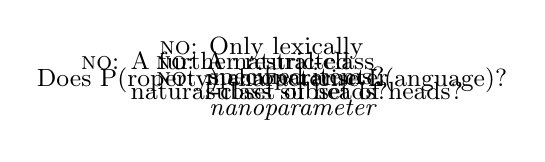
\begin{tikzpicture}[baseline=(root.base), font=\small]
        \tikzset{level 1/.style={sibling distance=-50pt}}
        \tikzset{level 2/.style={sibling distance=-60pt}}
        \tikzset{level 3/.style={sibling distance=-10pt}}
%        \tikzset{level 4/.style={sibling distance=-35pt}}
        \tikzset{level 3+/.style={level distance=50pt}}
%        \tikzset{level 4/.style={level distance=50pt}}
        \Tree   [.\node(root){Does P(roperty) characterise L(anguage)?};
                    {\textsc{yes}: \textit{macroparameter}}
                    [.\node(macro1){{\textsc{no}: macroparameter}};
                        {\textsc{yes}: \textit{macroparameter}}
                        [.\node[align=left](macro2){\textsc{no}: A natural-class\\
                                \strut\hphantom{\textsc{no}: }subset of heads?};
                            {\textsc{yes}: \textit{mesoparameter}}
                            [.\node[align=left](meso){\textsc{no}: A further restricted\\
                                \strut\hphantom{\textsc{no}: }natural-class
                                subset of heads?};
                            {\textsc{yes}: \textit{microparameter}}
                            \node[align=left](no){\textsc{no}: Only lexically\\
                                \strut\hphantom{\textsc{no}: }specified items?\\
                                \strut\hphantom{\textsc{no}: }\textit{nanoparameter}};
                            ]
                        ]
                    ]
                ]
    \end{tikzpicture}
\end{figure}

The central idea summarised in (\ref{ex:schifano:12.13}) and \figref{ex:schifano:12.14} is that a macroparametric effect
obtains when a given property holds for all relevant heads, and is therefore
easily set by the learner and likely to be stable over millennia. As one moves
downward the hierarchy, the subset of heads characterised by the relevant
property increasingly reduces, moving from a natural-class subset of heads (cf.
mesoparameter), through a further restricted natural-class subset of heads (cf.
microparameter), to a reduced set of lexically specified items (cf.
nanoparameter), all increasingly less salient in the \gls{PLD} and consequently less
resistant to reanalysis \parencite[261]{BibRob2016}.

Turning our attention again to the morpho-syntactic distribution of \emph{ben}
described above, which gradually decreases as one moves outside the productive
isogloss of Trentino (cf.\ Group 3 and 1, respectively), passing through a grey
area of variation (cf.\ Group 2), we immediately realise that this kind of
diatopic variation remarkably reflects the path of specialization predicted by
the above taxonomy. If we label the discourse function carried out by
\emph{ben} as \enquote{negative marking of negative presupposition}, as argued in
\textcite{CognSchi2018b}, we observe that in the early varieties discussed
above (here cumulatively referred to as \enquote{early Italo-Romance}) and in Trentino,
such marking is allowed on all [$+$V] heads, that is a natural-class subset of
heads, corresponding to a mesoparametric option. Conversely, Group 3 seems to
split its behaviour. As far as its lexical verbs are concerned, these clearly
instantiate a microparametric option, with \emph{ben} being attested in a
further restricted natural-class subset of heads, namely [$+$V] perfective heads
(cf.\ Restriction 2). Conversely, its functional (viz.\ restructuring) verbs
represent a nanoparametric choice, in that \emph{ben} seems to be allowed only
on lexically specified items (cf.\ \emph{potere} vs.\
\emph{smettere}).\footnote{The restrictions on the occurrence of \emph{ben} with
    restructuring verbs do not seem to be amenable to an alternative
    explanation to their nanoparametric classification proposed here. Indeed,
    the position of the tested restructuring verbs in \citegen{Cinque2006}
    hierarchy, which could plausibly play a role, does not seem to be relevant
    here, as \emph{volere}, which is the highest, is less accepted than
    \emph{potere}, which is the lowest, but \emph{smettere}, which lexicalises
    a position between the two, is largely ruled out (see also
\citealt{CognSchi2018}).} The relevant portion of this hierarchy is sketched
in \figref{ex:schifano:12.15}.

\begin{figure}
  \caption{The distribution of \emph{ben}\label{ex:schifano:12.15}}
    \hspace*{-.25cm}
    \begin{tikzpicture}[baseline, font=\small]
        \tikzset{level 1/.style={sibling distance=-55pt}}
        \tikzset{level 2/.style={sibling distance=-75pt}}
        \tikzset{level 3/.style={sibling distance=-25pt}}
        \tikzset{level 4/.style={sibling distance=-5pt}}
        \Tree   [.\node(root){};%\node[align=left]{Does the system mark negation of negative presupposition?};
                    {\textsc{no} (\textit{macroparameter})}
                    [.\node(macro1){{\textsc{yes}: on all heads?}};
                        {\textsc{yes}: (\textit{macroparameter})}
                        [.\node[align=left](macro2){\textsc{no}: on all [$+$V] heads?};
                            \node[align=left]{\textsc{yes}: early \ili{Italo-Romance} \emph{ben(e)}\\
                            \hphantom{\textsc{yes}: }Trentino \emph{ben}\\
                            \hphantom{\textsc{yes}: }\textit{mesoparameter}};
                            [.\node[align=left](meso){\textsc{no}: on all
                            [$+$V][$+$\Pfv] heads?};
                                \node[align=left]{%
                                    \textsc{yes}: Group 3 \emph{ben}\\
                                    \hphantom{\textsc{yes}: }(lexical verbs)\\
                                    \hphantom{\textsc{yes}: }\textit{microparameter}
                                };
                                \node[align=left](no){%
                                    \textsc{no}: on specific [$+$V] \\
                                    \hphantom{\textsc{no}: }heads? \\
                                    \hphantom{\textsc{no}: }Group 3 \emph{ben}\\
                                    \hphantom{\textsc{no}: }(restructuring verbs)\\
                                    \hphantom{\textsc{no}: }\textit{nanoparameter}
                                };
                                ]
                        ]
                    ]
                ]
        \node [above=-6mm of root, align=left]
            {Does the system mark negation\\
            of negative presupposition?};
    \end{tikzpicture}
\end{figure}

The fact that Group 3 simultaneously instantiates both a micro and
nanoparametric option or, more precisely, that lexical vs.\ functional verbs are
split in their behaviour, may be unexpected under the taxonomy in (\ref{ex:schifano:12.13}) and \figref{ex:schifano:12.14},
but finds a plausible explanation if we consider the diachrony. As discussed in
\Cref{sec:23-diachronic}, the distribution of \emph{ben} in Group 3 is likely to represent a
reduction of a previously much more extended usage, i.e.\ it is an instance of
diatopic variation which reflects a diachronic path. A closer look at the data
presented in \textcite{CognSchi2018b,CognSchi2018} suggests that such a
retraction may still be on-going.\footnote{For example, our investigation with
    native speakers has shown that there is a tendency for modally-marked
    compound tenses (e.g.\ conditional perfect) to score better than the
    temporally-related ones (e.g.\ present perfect).
%
%\begin{exe}
%    \exi{(i)}
%	\gll    Gianni avrebbe \textit{ben} comprato qualcosa, se avesse potuto.\\
%		    G. have.\Cond.\Tsg{} \textsc{ben} bought something if have.\Sbjv.\Ipfv.\Tsg{} been.able\\
%	\glt    \enquote*{Gianni would have bought something, if he had been able to.}
%\end{exe}
%
%\begin{exe}
%    \exi{(ii)}
%	\gll    Gianni ha \textit{ben} comprato qualcosa.\\
%		    G. have.\Prs.\Tsg{} \textsc{ben} bought something\\
%	\glt    \enquote*{Gianni has bought something.}
%\end{exe}
%
Similarly, if a compound form allows both a temporal and a modal reading (e.g.\
future perfect with temporal vs.\ epistemic interpretation), the
latter is usually preferred.

%\begin{exe}
%    \exi{(iii)}
%	\gll Gianni avrà \textit{ben} comprato qualcosa per quando noi torniamo.\\
%		G. have.\Fut.\Tsg{} \textsc{ben} bought something for when we return.\Prs{}.\Fpl{}\\
%	\glt \enquote*{Gianni will have bought something by the time we come back.}
%\end{exe}
%
%\begin{exe}
%    \exi{(iv)}
%	\gll Gianni avrà \textit{ben} comprato qualcosa, immagino.\\
%		G. have.\Fut.\Tsg{} \textsc{ben} bought something imagine.\Prs.\Fsg{}\\
%	\glt \enquote*{Gianni will have bought something, I believe.}
%\end{exe}

This further and rather subtle specialization with compound tenses (i.e.\ the
only morpho-syntactic combination allowed with lexical verbs), not necessarily
shared by all speakers yet, may indicate that the retraction of \emph{ben} in
Group 3 is still on its way. See \citet{CognSchi2015} for data showing a
similar tendency with \emph{smettere} (i.e.\ largely ruled out, but
modally-marked interpretations receive higher scores).} Under this hypothesis,
the behaviour of Group 3 and the representation in \figref{ex:schifano:12.15} are no longer
surprising. That the lower branches represent unstable options is indeed
consistent with current assumptions on diachronic change within the parametric
hierarchy approach, where micro-\is{parameters} and nanoparametric options are taken to be
highly unstable \parencite[261]{BibRob2016}.

\section{Conclusions}\label{sec:23-conclusions}

In the present squib we have discussed the distribution of the discourse
particle \emph{ben} in a selection of regional varieties of \ili{Italian}, as
described in \textcite{CognSchi2015,CognSchi2018b,CognSchi2018}. On the basis
of the judgements expressed by native speakers, we have identified three main
morpho-syntactic restrictions which affect the distribution of \emph{ben} in
Group 3 but not in Group 1, which we take to be the productive isogloss. A
preliminary examination of diachronic evidence has also suggested that the more
liberal use of Trentino reflects an earlier stage of \ili{Italo-Romance}, where
\emph{ben} was also allowed in wide array of TAM-contexts. In conclusion, we
have suggested that the attested diatopic variation can be successfully
formalised in terms of a parameter hierarchy, in that the gradual retraction of
the admitted contexts we described finds a remarkable parallel with the macro >
meso > micro > nano path independently argued for by the parametric hierarchy
approach on the basis of extensive diachronic and typological evidence. This
also allows us to provide new insights into the diachronic development of
\emph{ben} from early \ili{Italo-Romance} to present-day varieties. The advantage of
modelling the (shrinking) diatopic and diachronic distribution of \emph{ben}
via a parameter hierarchy is that it allows us to formally capture a type of
variation which would otherwise look like random change (see for example the
\emph{potere} vs.\ \emph{volere} restriction, here captured as a nanoparametric
option). The case of \ili{Italian} \emph{ben} also opens the way to future research
on the possibility that the (morpho-syntactic) behaviour of elements at the
syntax-discourse interface is also subject to the predictions of parametric
hierarchy approach.

\printchapterglossary{}

\section*{Acknowledgements}

We would like to dedicate this squib to Ian Roberts, whose work and outstanding
scholarship has greatly inspired our own investigations. We hope that it is
successful in showing how his research, including the one conducted with the
\emph{ReCoS} team, is opening the way to new thrilling lines of investigation.

Although this entire work stems from joint research, for the administrative
purposes of the \ili{Italian} academia Norma Schifano takes responsibility for §1,
§2 and §4 and Federica Cognola for §3 and §5.

\nocite{IlNovellino,Monumenti}
\printbibliography[heading=subbibliography, title={Sources},
keyword={23-source}]

{\sloppy
\printbibliography[heading=subbibliography,notkeyword=this,notkeyword=23-source]
}

\end{document}
